\chapter{Results}
\label{chap:results}
We expect that the \gls{wdt} method will improve the statistics of
Serpent 2 calculations. With normal delta-tracking, virtual collisions
provide no statistical benefit, and are therefore an inefficient use
of computational resources. Virtual collisions that results in
absorption events do contribute to statistics when using
\gls{wdt}. Therefore, we expect an improvement in the results of a
Serpent 2 simulation. In this section, we will describe how
performance in Serpent 2 is quantified, describe the three test cases,
and the results of those test cases.

\section{Performance metrics}
\label{sec:fom}

\subsection{Figure of Merit}
\label{sec:fom}

Monte Carlo codes such as Serpent 2 run many batches of a single
simulation, calculating the mean of values of interest $\hat{x}$
across the many runs. By the central limit theorem, we know that the
means across many simulations will form a normal distribution with
variance $\sigma^2(\hat{x})$. We are interested in reducing the
variance of the final value which will provide more confidence in the
simulation results. In general, running the simulation more times will
reduce this variance at the cost of requiring more computation
time. The variance is proportional to the number of cycles $n$:
\begin{equation}
\label{eq:variance}
  \sigma^2(\hat{x}) = \frac{C}{n}
\end{equation}
Therefore, when we seek to improve the quality of the
statistics, as with \gls{wdt}, we are seeking improved variance with
less cycles. To measure this, we must establish a \gls{fom}.
The standard \gls{fom} used by most simulations, described by Lewis
and Miller~\cite{lewis1993}, is shown in Eq.~\eqref{eq:fom}:
\begin{equation}
  \label{eq:fom}
  \mathrm{FOM} = \frac{1}{\sigma(\hat{x})^2T}
\end{equation}
where $T$ is the runtime of the simulation, $T = Cn$. The runtime is
proportional to the number of cycles $n$, plugging in
Eq.~\eqref{eq:variance}:
\begin{equation*}
  \mathrm{FOM} = \frac{1}{\sigma(\hat{x})^2T}} = \frac{C\cdot n}{n} = C
\end{equation*}


 A higher \gls{fom}
indicates higher accuracy per computation time, and therefore a more
efficient algorithm. Serpent 2 collects scores for each cycle (or
batch of cycles) and outputs the sample mean and standard
deviation\todo{Check if this is stdev or
  var}~\cite{VTT-R-00371-14}. This enables comparison of Serpent 2
running with and without \gls{wdt} to determine the efficiency of the
algorithm.

\subsection{Convergence}
\label{sec:convergence}

As described in the previous section, we expect the variance to
improve with further simulation. Fig.~\ref{fig:error_convergence}
shows the variance in the measurement of infinite flux,
$\phi_{\infty}$ as a function of Serpent 2 simulation cycles. As
shown, the variance decreases linearly as the simulation is run
further.
\begin{figure}[hbtp]
  \centering
  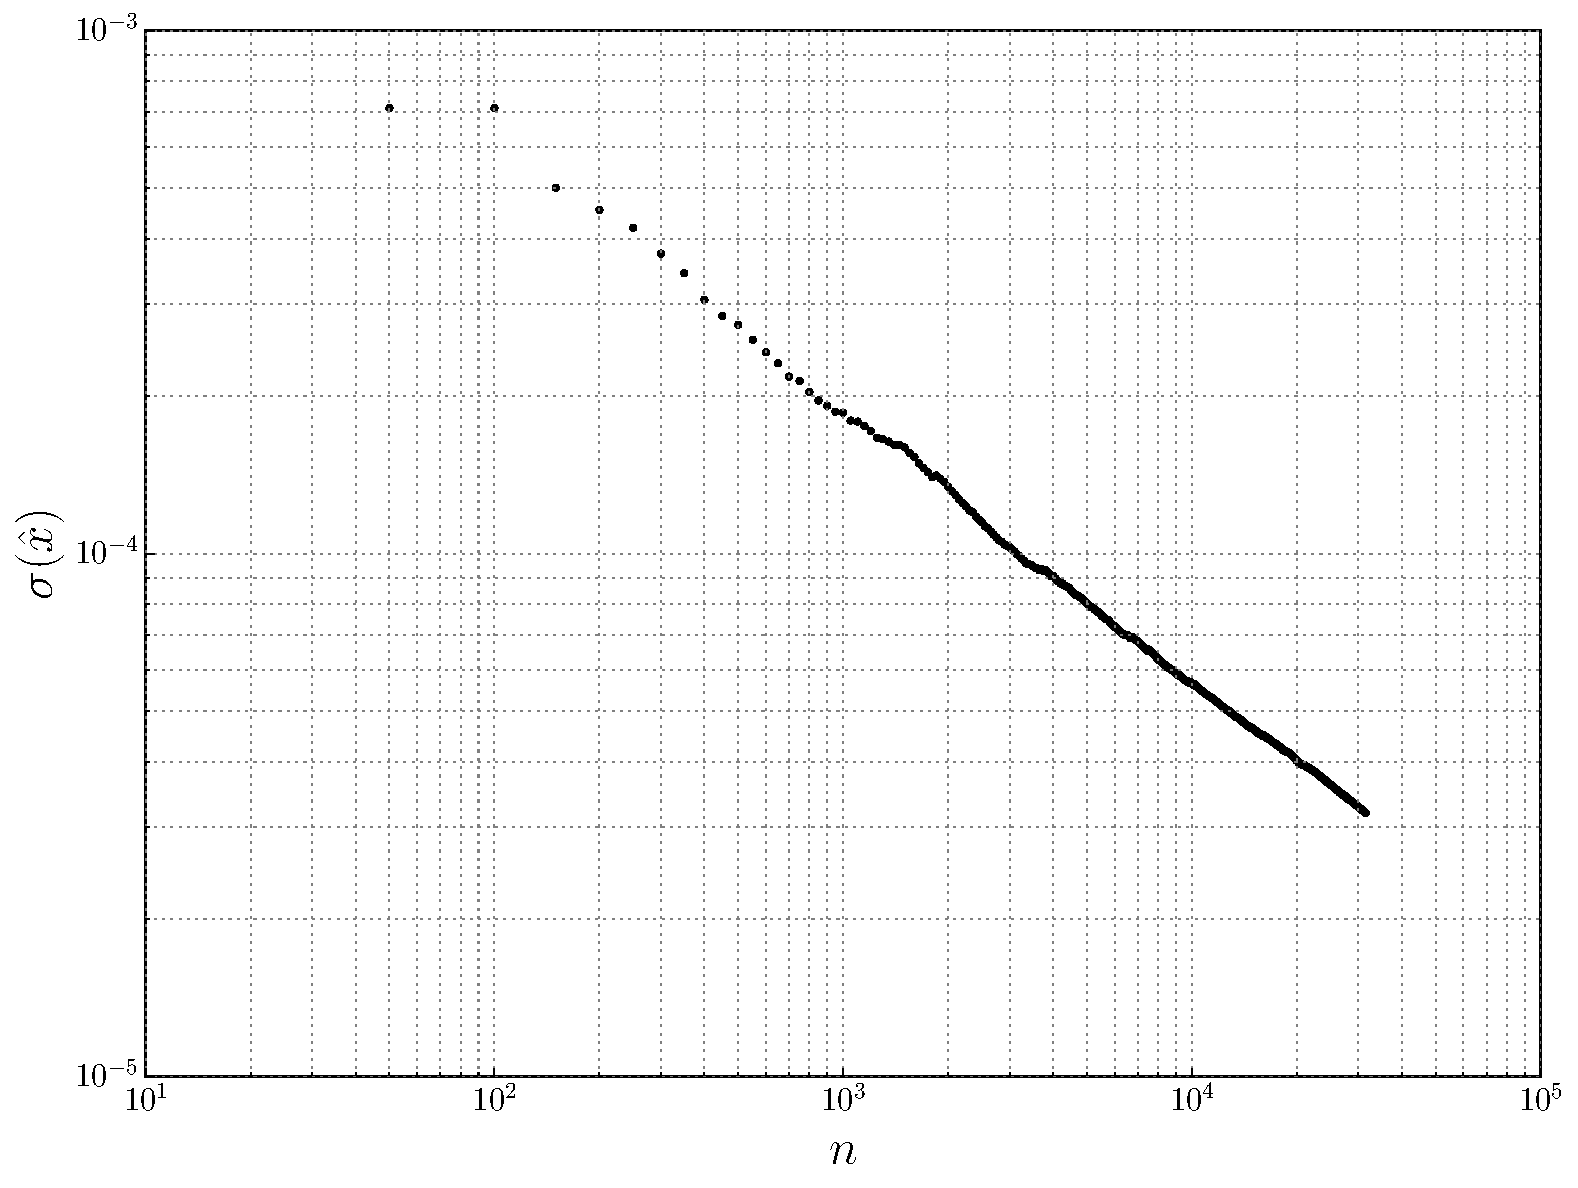
\includegraphics[scale=0.4]{images/error_convergence}
  \caption[Variance in $\phi_{\infty}$ for the fast-neutron group as a
    function of Serpent 2 cycle.]{Variance in $\phi_{\infty}$ for the fast-neutron group as a
    function of Serpent 2 cycle, with \gls{wdt} threshold of 0.2.}
  \label{fig:error_convergence}
\end{figure}

\begin{figure}[hbtp]
  \centering
  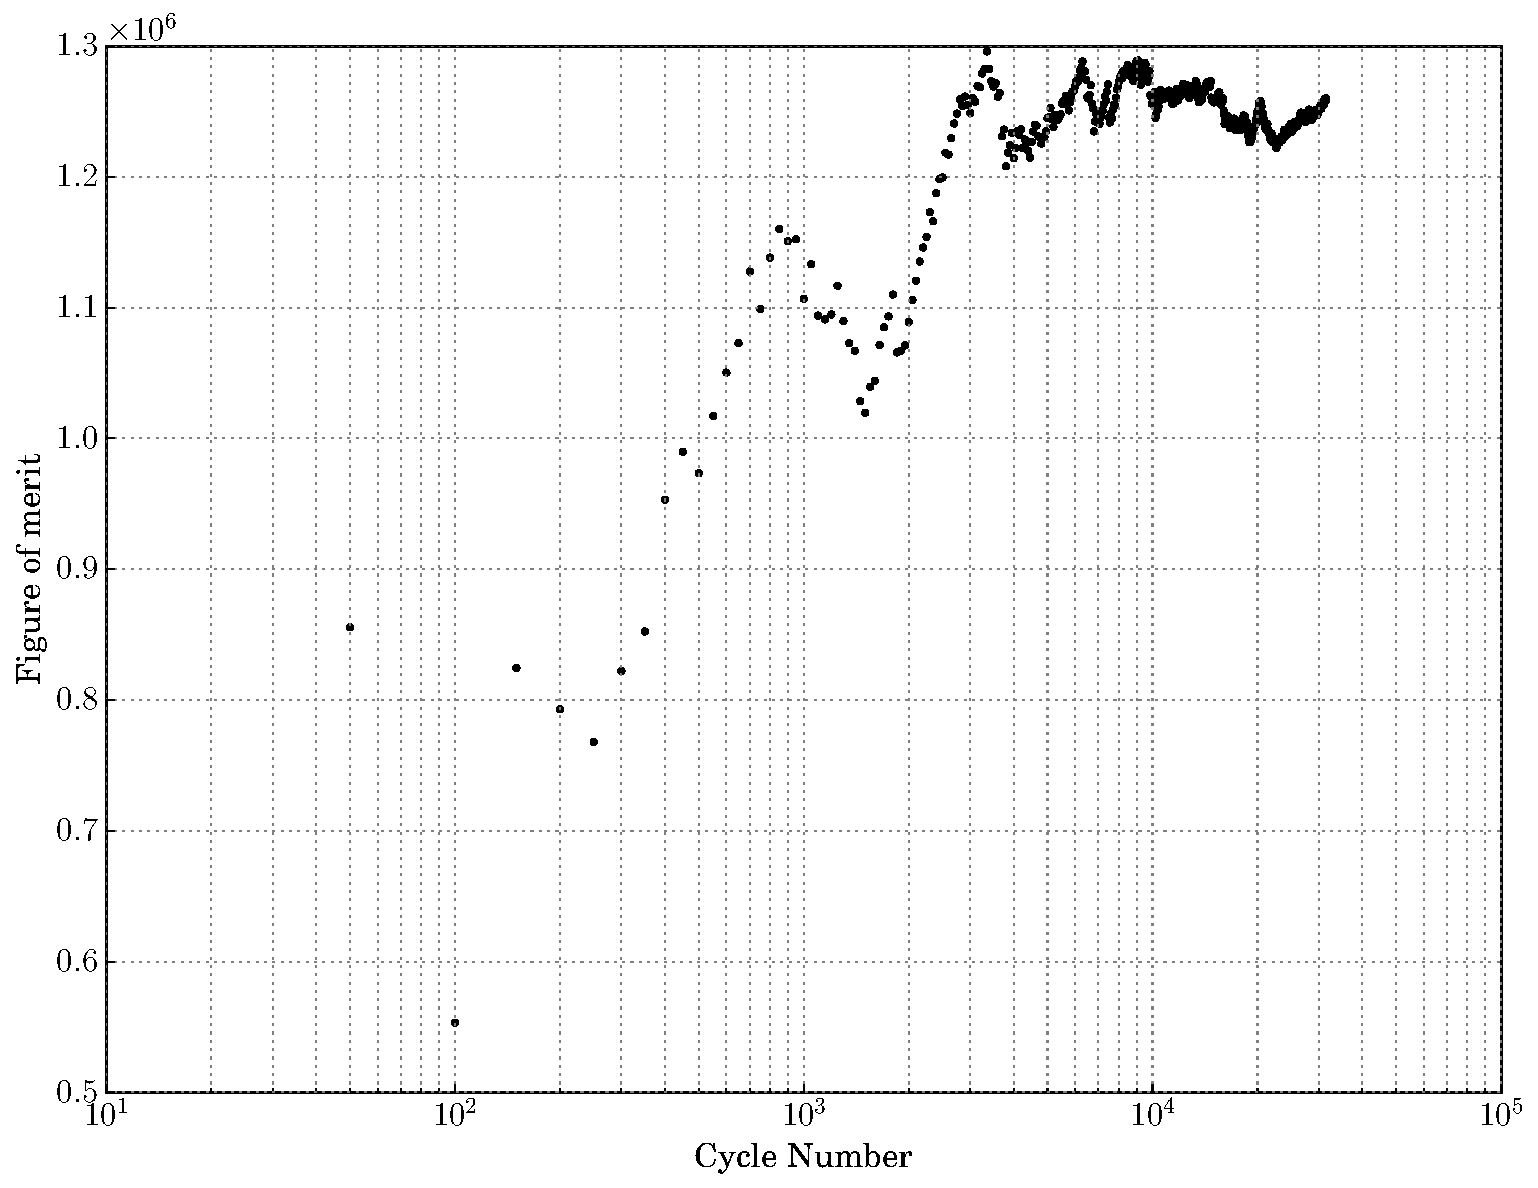
\includegraphics[scale=0.4]{images/fom_convergence_example}
  \caption[Figure of merit in $\phi_{\infty}$ for the fast-neutron group as a
    function of Serpent 2 cycle.]{Figure of merti in $\phi_{\infty}$ for the fast-neutron group as a
    function of Serpent 2 cycle, with \gls{wdt} threshold of 0.2.}
  \label{fig:fom_convergence}
\end{figure}

%% Convergence explanation

% Test Cases

%% PWR
%% Fast Pincell
%% Homog Element

%% -- Images

% Actual Results

%% Infinite flux

%% Cross-sections

%% Scattering matrices

%%% Local Variables:
%%% mode: latex
%%% TeX-master: "../masters_report"
%%% End:
